\documentclass{standalone}
\usepackage[english]{babel}
\usepackage{etoolbox} % for "textbf" command
\usepackage[dvipsnames]{xcolor}
\usepackage{tikz}
\usetikzlibrary{shadows.blur}
\usetikzlibrary{shapes.symbols}
\usetikzlibrary{calc} % for arithmetic
\usetikzlibrary{shapes.geometric} % for polygons

\newcommand{\len}[1]{\vert#1\vert}
\newcommand{\TT}[1]{\texttt{#1}}
\newcommand{\BF}[1]{\textbf{#1}}

\definecolor{snow}{RGB}{238,233,233}

\begin{document}

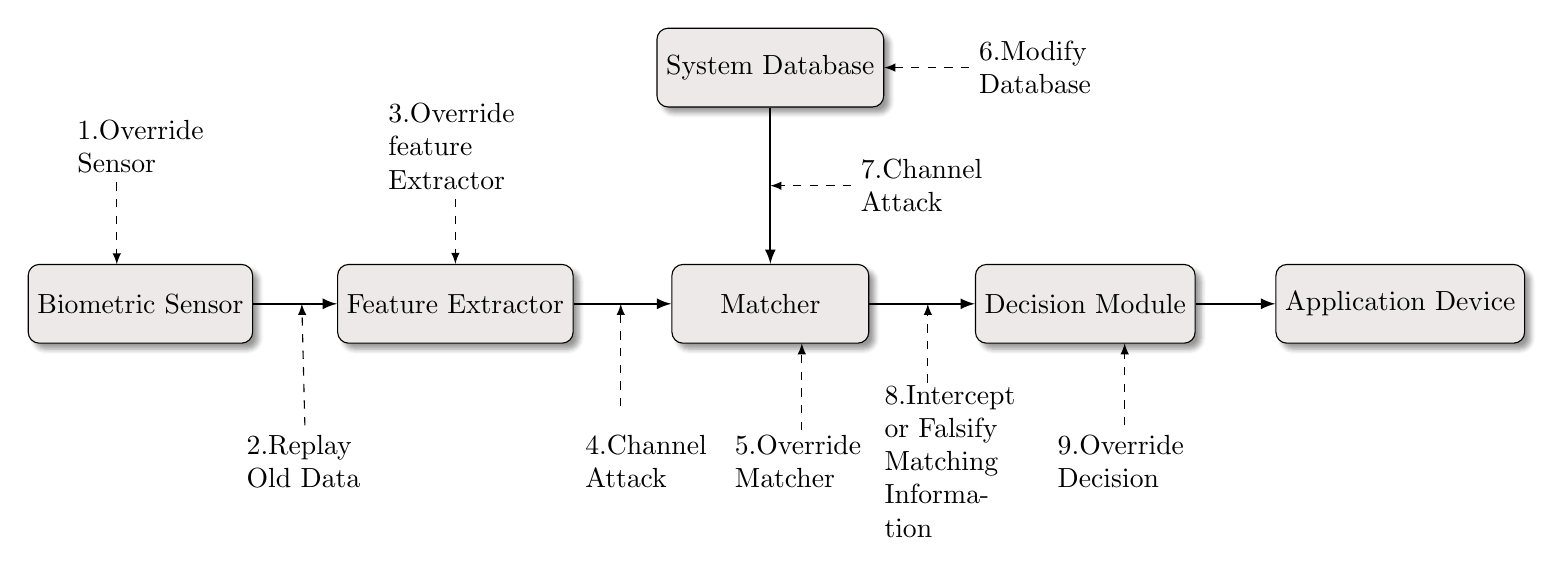
\begin{tikzpicture}
\tikzstyle{lelement}=[rectangle,rounded corners,blur shadow={shadow blur steps=5,shadow blur extra rounding=1.5pt},draw,fill=white,minimum height=1cm, minimum width=2.5cm]

\node [lelement, fill=snow] (A) at (-2,0) {Biometric Sensor};
\node [lelement, fill=snow] (B) at (2,0) {Feature Extractor};
\node [lelement, fill=snow] (C) at (6,0) {Matcher};
\node [lelement, fill=snow] (D) at (6,3) {System Database};
\node [lelement, fill=snow] (E) at (10,0) {Decision Module};
\node [lelement, fill=snow] (F) at (14,0) {Application Device};

\draw[->,thick,rounded corners,>=latex] (A) -- (B);
\draw[->,thick,rounded corners,>=latex] (B) -- (C);
\draw[->,thick,rounded corners,>=latex] (D) -- (C);
\draw[->,thick,rounded corners,>=latex] (C) -- (E);
\draw[->,thick,rounded corners,>=latex] (E) -- (F);

\node [text width=1cm  ] (1) at (-2.3,2) {1.Override Sensor};
\node [text width=1.5cm] (2) at (0.1,-2) {2.Replay Old Data};
\node [text width=1.7cm] (3) at (2,2) {3.Override feature Extractor};
\node [text width=1.7cm] (4) at (4.5,-2) {4.Channel Attack};
\node [text width=1.7cm] (5) at (6.4,-2) {5.Override Matcher};
\node [text width=1.7cm] (6) at (9.5,3) {6.Modify Database};
\node [text width=1.7cm] (7) at (8,1.5) {7.Channel Attack};
\node [text width=1.7cm] (8) at (8.3,-2) {8.Intercept or Falsify Matching Information};
\node [text width=1.7cm] (9) at (10.5,-2) {9.Override Decision};

\draw[->,dashed,rounded corners,>=latex] (1) -- (-2.3,0.5);
\draw[->,dashed,rounded corners,>=latex] (2) -- (0.05,0);
\draw[->,dashed,rounded corners,>=latex] (3) -- (B);
\draw[->,dashed,rounded corners,>=latex] (4.1,-1.3) -- (4.1,0);
\draw[->,dashed,rounded corners,>=latex] (6.4,-1.6) -- (6.4,-0.5);
\draw[->,dashed,rounded corners,>=latex] (6) -- (D);
\draw[->,dashed,rounded corners,>=latex] (7) -- (6,1.5);
\draw[->,dashed,rounded corners,>=latex] (8,-1) -- (8,0);
\draw[->,dashed,rounded corners,>=latex] (9) -- (10.5,-0.5);


\end{tikzpicture}

\end{document}